\section{Introduction }
\label{sec:introduction}

\subsection{Background}
\label{subsec:background}

A rumor is defined as a ``proposition for belief of topical reference disseminated without official verification,''~\cite{knapp-1944} a notion that lends itself quite well to the imagination of applied mathematicians.
The mathematics of rumor spread is somewhat explored, beginning with the epidemic model applied to information spread in a population by Daley and Kendall in 1965.
This model's assumptions of homogeneous interactions and its lack of well-defined parameters likely caused ``the superficial similarity between rumors and epidemics to break down on closer scrutiny''~\cite{daley-1965}.
Nonetheless, the similarities of knowing and spreading a rumor, and having and spreading a disease, share parallels that only deviate in some of the intricacies of their mechanism.
In both, an ``infected'' individual in a network desires to (or inadvertently spreads) their ``condition.''
With disease, one of the mechanisms of suppressing spread is vaccination; with rumors it is an individual's eventual boredom and desire for novel information.

More recent models of rumor spread in a population examined the dynamics through randomized networks~\cite{karp-2000}, examining the rumor transmission in exponentially distributed networks~\cite{moreno-2004}, and the time of rumor spread given contacts of the initial spreader in a regular network~\cite{fount-2010}.
There is increasing emphasis on the structure of networks themselves and how this affects model dynamics~\cite{zhang-2013, pellis-2015, pellis-2012, ball-2010, zhou-2007}.
Many of these models derive their structure and dynamics from complex yet internally homogeneous simulations of how individuals interact with rumors.
However, with the advent social media and their massive networks that allow sharing of information on a large scale, more analyses focus on frequently-found behaviors on these platforms.
Simulations of rumor spread through social media are becoming increasingly realistic by including ``forgetting'' mechanisms typical of social media~\cite{zhao-2011}, comparing time of rumor spread in random networks as compared to structured networks~\cite{liu-2011}, methods for combatting rumor spread in social networks~\cite{tripathy-2010}, and examining rumor spread on gaming networks~\cite{grab-2008}.

\subsection{The ISTK Model}
\label{subsec:istk}

In this paper we consider a rumor spread model with four categories of individuals: the ``ignorant'' individuals, those who have never heard the rumor; the ``spreaders,'' those that have heard the rumor and are actively spreading it; the ``stiflers,'' those who have heard the rumor and actively suppress further transmission (either because they now consider the rumor old news, or they never believed the rumor in the first place); and finally the ``knowledgeable'' population, those who have heard, but have subsequently forgotten the rumor.
The rumor initializes in only a small fraction of the population, and spreads as the individuals interact.
The ignorant, spreader, and stifler populations were presented in the Daley-Kendall (DK) model~\cite{daley-1965}, but it had been postulated that a distinct ``knowledgeable'' population was necessary~\cite{zhao-2012, zhao-2011}.
Assuming otherwise presumes that the attitude of an individual who has forgotten a rumor is identical to the behavior of an individual who had not yet heard the rumor.
We account for this distinction with the addition of the knowledgeable population to the DK model.
We dub this updated model the Ignorant, Spreader, Stifler, and Knowledgeable (ISTK) model.

We use three variations of this model: one differential, and two agent-based.
The differential ISTK model simulates a homogenous group of people, and has no awareness of the concept of individuals; it simply ``moves'' proportions of the group of people from one population to another over time.
The first agent-based model, the ``simple model,'' simulates individuals through several iterations (rounds) over time.
The model incorporates a network that represents the connections between individuals, which in this case is based off of Facebook friends.
The second agent-based model, the ``feature-vector model,'' incorporates demographic data of these Facebook users.

In the feature vector model, we further consider how a rumor might be targeted towards certain individuals.
Instead of assuming that every individual is equally likely to spread a rumor, we assumed that certain characteristics of the rumor and of the individual affect the likelihood of the individual to spread the rumor.
This idea is supported by evidence that suggests that people are more likely to believe information that comes from others with similar values~\cite{gillespie-2004}.
Serendipitously, the original social network dataset included demographic data, like education level, gender, and language.
Therefore, we decided to use demographics of the individuals as their ``features'' and that a rumor could be targeted to appeal to certain demographics.
While an individual's response to viral information is certainly more complex, our underlying assumption is simply that a rumor \textit{can} be targeted towards an individual.
Demographic information seemed like a reasonable way to equip individuals and rumors with these features.
We call this feature vector the ``personality'' of the rumor.
Moreover, we can compute a notion of ``similarity'' between the feature vector of the rumor and that of an individual.
In this way, the more similar an individual and rumor were, the more likely an individual would spread the rumor.
This effect is also suggested by the theory of confirmation bias, insofar as we are more likely to accept information that confirms our previous beliefs~\cite{wason-1960}.

\subsection{ISTK Model Equations}
\label{subsec:istkeqns}

\begin{figure}[H]
\captionsetup{width=0.6\textwidth}
\centering
    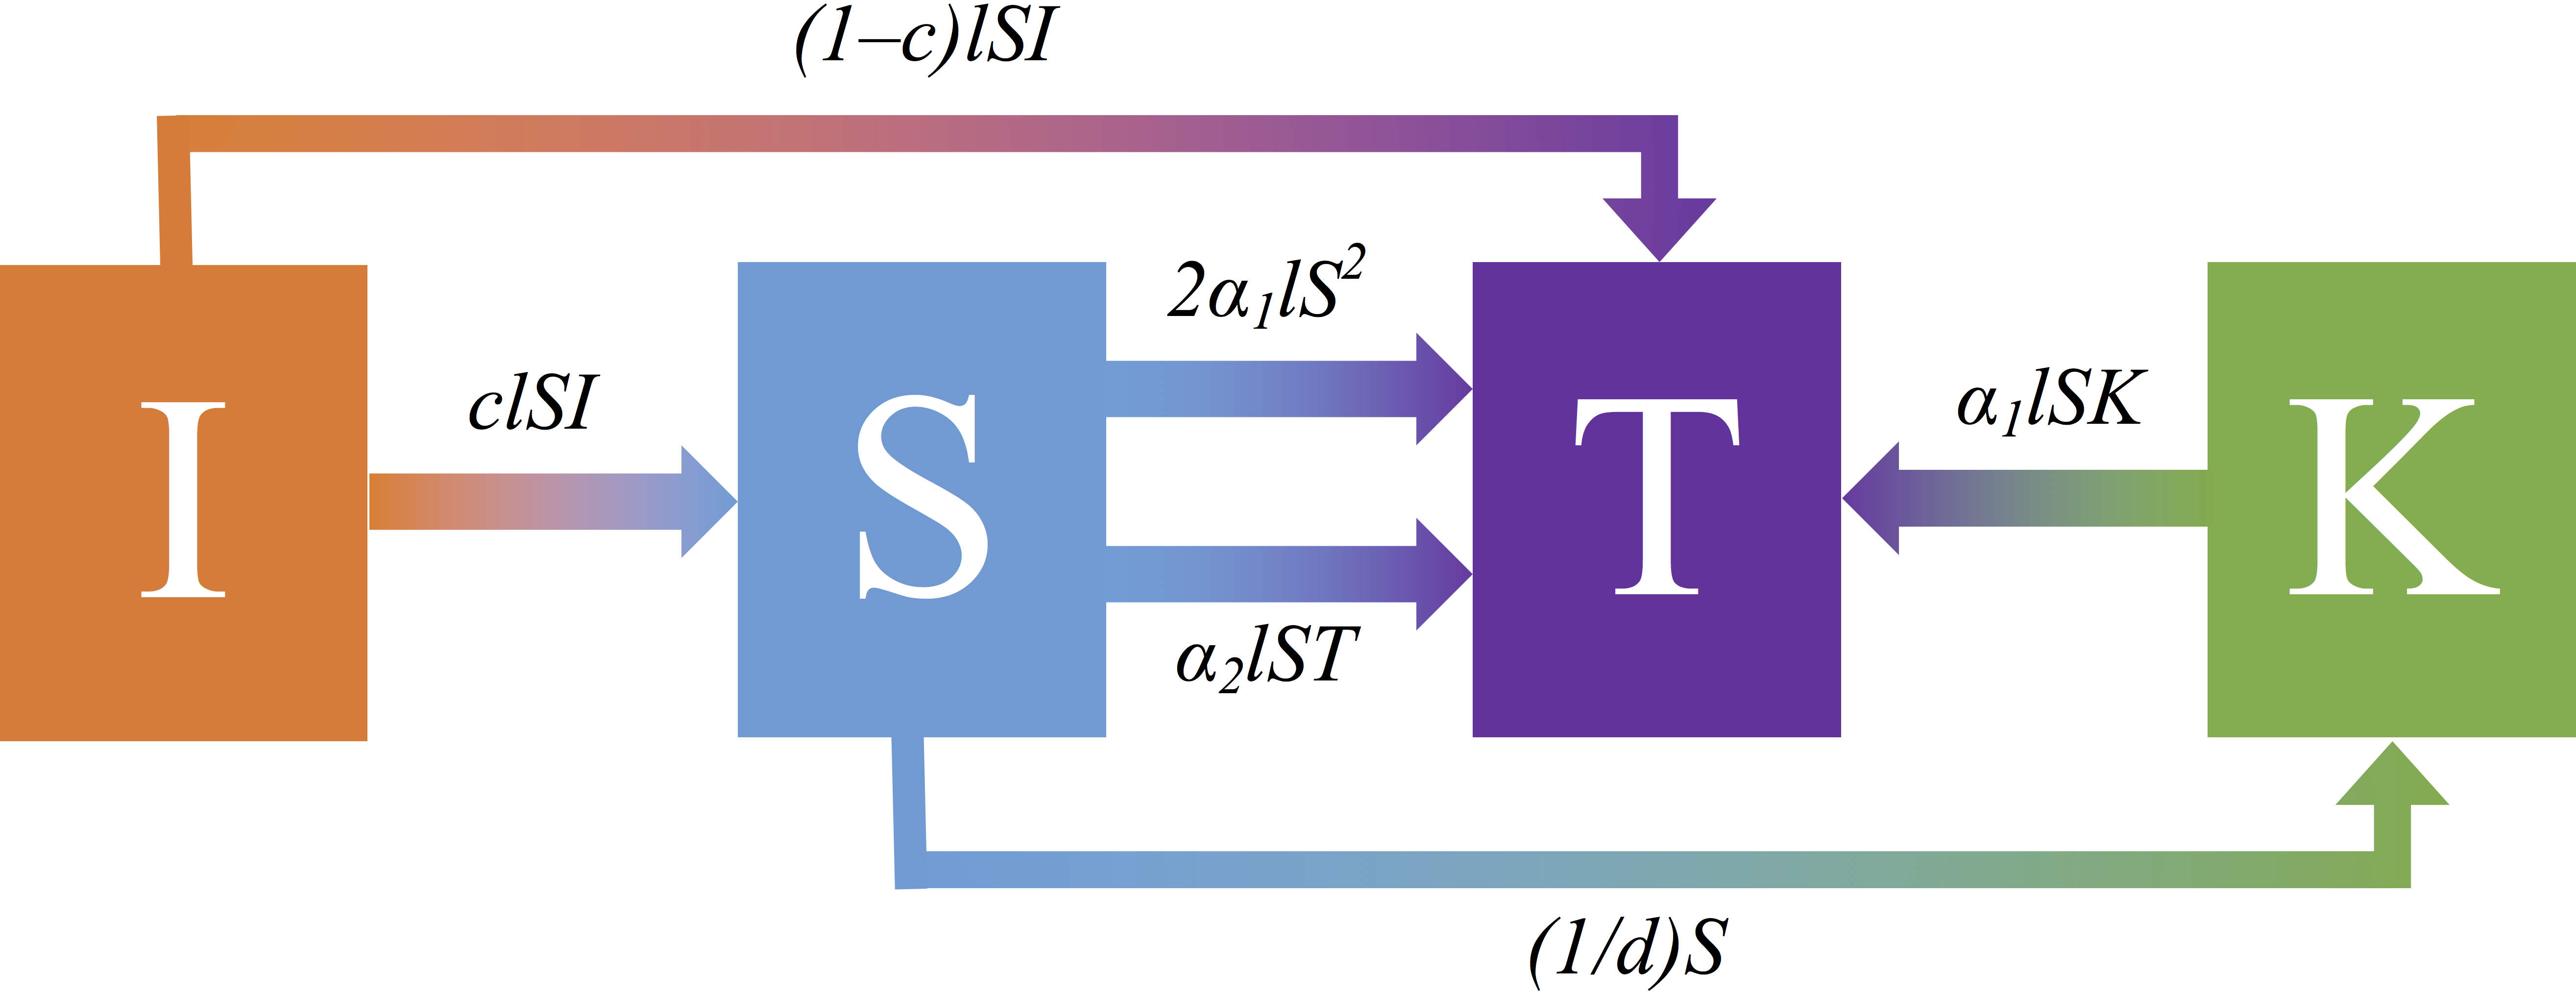
\includegraphics[width=0.85\textwidth]{figures/flow-chart}
  \caption{The ISTK Model, a flowchart}
\label{fig:flow-chart}
\end{figure}

\noindent Figure~\ref{fig:flow-chart} represents how individuals can move from one population to another.
The base of each arrow represents the population an individual moves from, while the head represents the population an individual moves to.
The labels for each arrow express the parameters that control that particular mechanism for moving individuals between the two populations. These labels include two distinct parts. First, some lowercase parameters, like $ c $ or $ l $, which are external factors that influence the rumor spread. Second, uppercase populations, which factor in the size of the corresponding population.

$ I $, $ S $, $ T $, and $ K $, represent the total Ignorant, Spreader, Stifler, and Knowledgeable populations respectively. The total size of the population is represented as $ N $, in that $ N = I + S + T + K $ (n.b.\ we assume no one dies or is born, so N stays constant, i.e. $\frac{dN}{dt} = 0$).

The parameters are as follows:
\begin{itemize}
    \item the ``credibility'' of the rumor, $ c $, expressed as a probability that an Ignorant believes the Spreader
    \item $ (1 - c) $\, the complement of $ c $, equivalent to being incredulous of the rumor
    \item $ l $, the chance per day of interaction, which is the complement of the overall probability that an individual does not talk with a single Spreader: it is computed by a set of Bernoulli trials with success probability $ \rho $ where $ \rho = 1 - \frac{S}{N} $ and number of trials to be $ \tau $ (i.e.~$ l = 1 - \rho^\tau $)
    \item $ d $, the number of days after which an individual forgets a rumor
    \item $ \alpha_1 $, the loss of novelty of the rumor
    \item $ \alpha_2 $, the chance that the Spreader becomes a Stifler upon interacting with a Stifler
\end{itemize}

In this way, each label represents the ``chance'' per day that an individual can move from one population to another. For example, the arrow that connects the I and T population with the label $ (1-c)SI $ reads: the chance an Ignorant becomes a Stifler is proportionate to their incredulity, the chance per day of interacting with a Spreader, and the size of the Spreader and Ignorant populations.

The model can be surmised by four differential equations, as follows:

\begin{equation}
\label{eqn:istk_exp_i}
\frac{dI}{dt} = - clSI - (1-c)lSI \\
\end{equation}

\noindent In Equation~\ref{eqn:istk_exp_i}, the first term describes the interaction between an Ignorant and a Spreader, which moves individuals to the Spreader population depending on the credibility of the rumor.
 The second term of Equation~\ref{eqn:istk_exp_i} accounts for being ``incredulous'' of the rumor, which moves Ignorants to Stiflers. (n.b.\ simplifying this equation to ($-lSI$) does not allow us to distinguish the credulous ($ c $) and incredulous ($ 1 - c $) group of people.)

\begin{equation}
\label{eqn:istk_exp_s} \frac{dS}{dt} = clSI - \frac{1}{d} S - 2 \alpha_1l S^2 - \alpha_2 ST \\
\end{equation}

The first term of Equation~\ref{eqn:istk_exp_s} is the addition of members from the Ignorant class who believed the rumor.
The second term $ \frac{1}{d} $, the inverse of the number of days it takes to forget the rumor, represents in the chance per day to forget the rumor.
The third term of Equation~\ref{eqn:istk_exp_s} accounts for two Spreaders who interact with each other and foster disinterest in the rumor (since the rumor has lost its novelty).
When these two Spreaders interact ($ S^2 $), we account for the chance that \textbf{each} Spreader could become a Stifler by multiplying the term by $ 2 $.
The final term represents the disillusionment power of a Stifler when interacting with a Spreader.

\begin{equation}
\label{eqn:istk_exp_t} \frac{dT}{dt} = 2 \alpha_1l S^2 + \alpha_1l SK + \alpha_2 ST + (1-c)lSI \\
\end{equation}

In equation~\ref{eqn:istk_exp_t}, the first term describes the transition from Spreader to Stifler.
The second term describes the population of Knowledgeable individuals who become a Stifler, as described in Equation~\ref{eqn:istk_exp_s}.
The third and fourth terms of Equation~\ref{eqn:istk_exp_t} describe the addition of members to the Stifler population from the Spreader and Ignorant populations, respectively.

\begin{equation}
\label{eqn:istk_exp_k} \frac{dK}{dt} = \frac{1}{d}S - \alpha_1l SK
\end{equation}

Finally, Equation~\ref{eqn:istk_exp_k} describes the individuals in the Spreader class who forget the rumor and become Knowledgeable; and the population which loses the novelty of the rumor and become Stiflers.

In our model, we do not consider the interaction between a Stifler and an Ignorant because neither one has a reason to broach the subject of a rumor (the Ignorant because they do not know and the Stifler because they no longer care).
Moreover, by a similar logic, when a Knowledgeable and Stifler interact, there is no change in populations.

Even more than the addition of the Knowledgeable population, our model differs from the Daley-Kendall (DK) model~\cite{daley-1965} by adding the parameter $ c $.
This parameter allows us to avoid the assumption that every individual believes the rumor upon hearing it.
Furthermore, the DK model permits individuals to return to the Ignorant class, which we also cannot happen in our model. Ignorant individuals are individuals who have truly never heard the rumor.
